\section{Timing layers for single particles}

Before considering the full Geant4 simulation, let us discuss the benefit of the TOF information
for identification of separate particles. Fig.~\ref{fig:singleparticles} shows the $3\sigma$ separation from the pion
mass hypothesis using the same procedure as discussed  in \cite{Cerri:2018rkm}. The 
calculations are performed for several options for the resolution of the timing layer, from 10~ps to 1~ns,
as a function of the travel length $L$ and the momenta. For a 20~ps detector and  for a typical travel 
distance of $L\sim 0.2$~m from the interaction point to the 
electromagnetic calorimeter, neutrons (and protons) can be separated from the pion hypothesis up to 7~GeV. The separation of $K-$mesons can be performed up to 3~GeV.
This momentum range should be sufficient for reliable particle identification in a wide range 
of physics studies, especially if such identification is used for jets that are dominated
by this momentum range of separate particles.
For a detector  with 1~ns, the separation can only be possible  up to  300 -- 500~MeV. This is below  than a typical
minimum transverse momentum of 0.5 -- 1~GeV for particles considered for high-energy proton colliders .
Therefore, a timing layer with 1~ns resolution cannot effectively be used for particle identification in such experiments.

\begin{figure}
\begin{center}
   \subfigure[Neutrons] {
   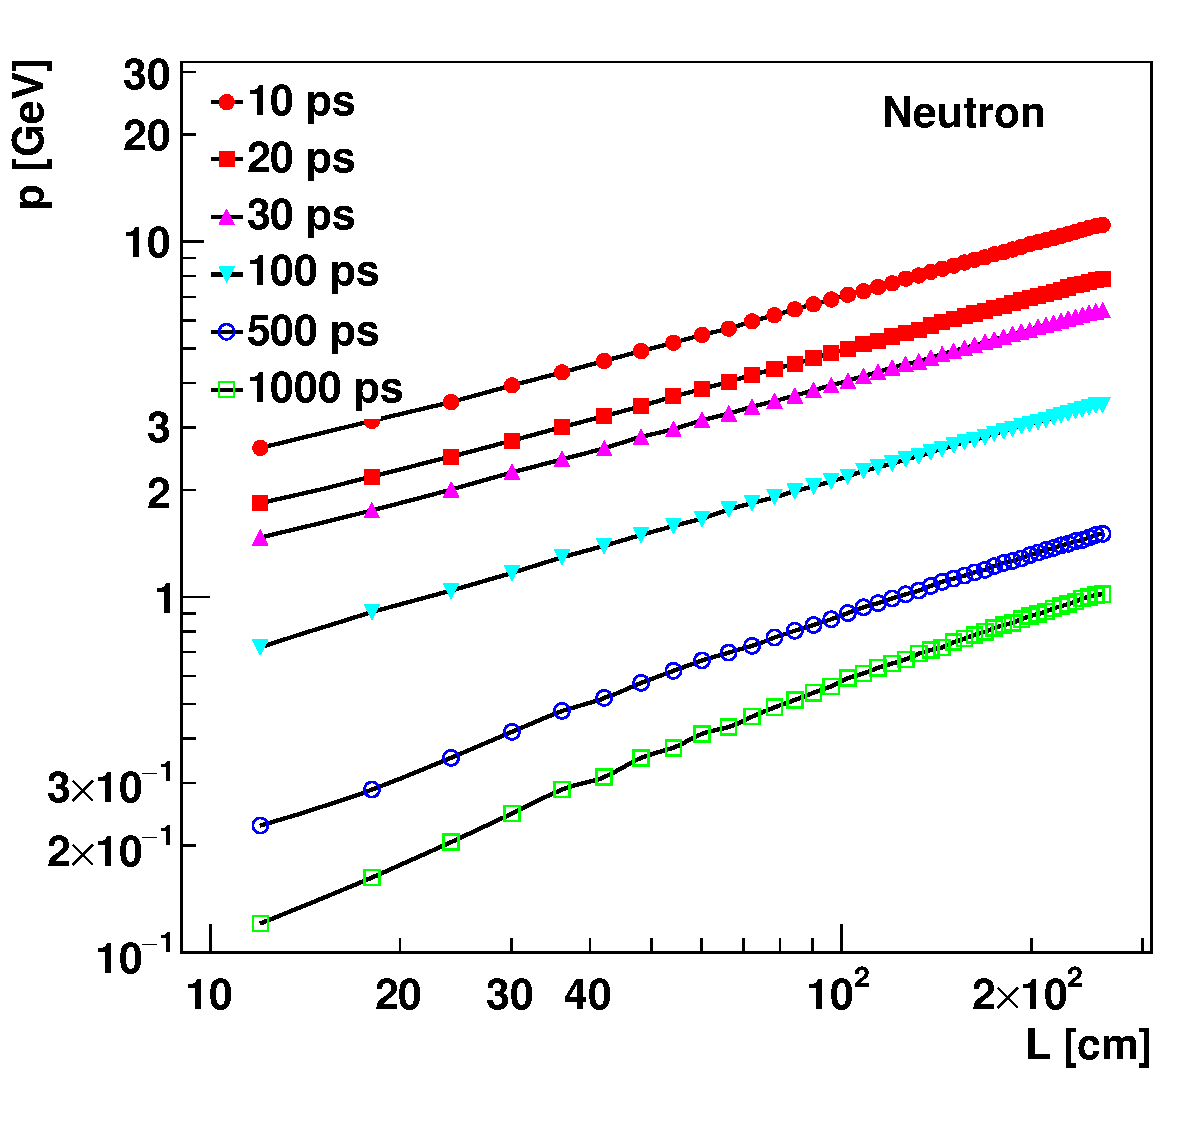
\includegraphics[width=0.6\textwidth]{time_flight_length_neutron.pdf}
   }
      \subfigure[$K$-mesons] {
   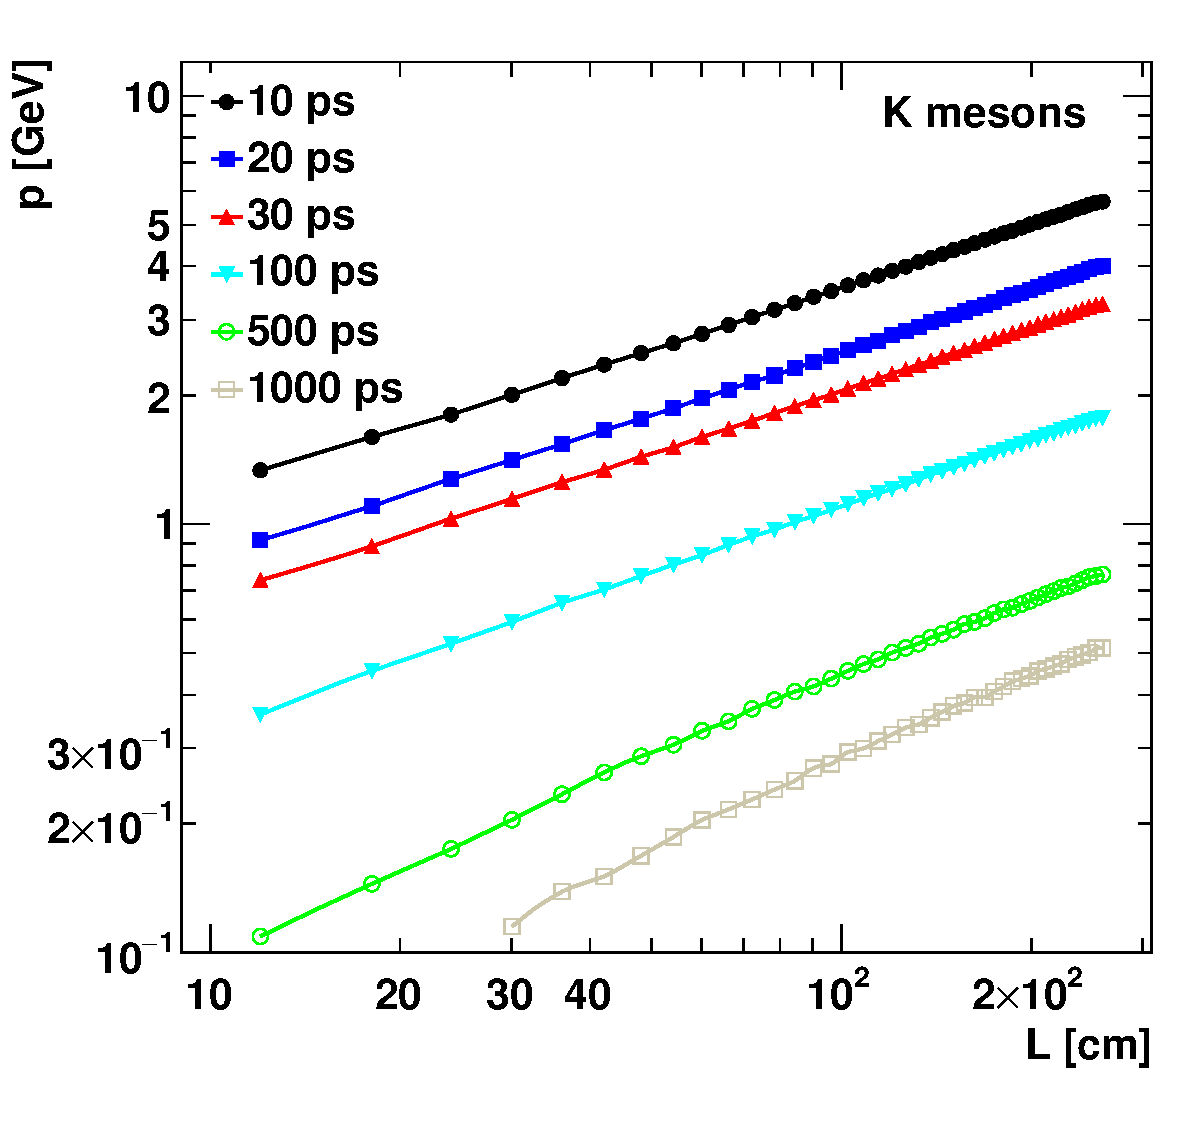
\includegraphics[width=0.6\textwidth]{time_flight_length_kion.pdf}\hfill
   }
\end{center}
\caption{
The $3\sigma$ separation from the pion mass for neutrons and $K$-mesons as a function of the distance and the momenta.
}
\label{fig:singleparticles}
\end{figure}


